\chapter{Results and Conclusion}\label{chap:results}
The algorithm described in \autoref{chap:algorithm} has also been tested in the real robot cell. As in the case of the simulation, two videos of the result can be found in the attachment. \autoref{fig:results} shows a frame of one of the videos. In \autoref{fig:results}, the robot is building a Bart figure and it has already built a Homer and a Marge.

\begin{figure}[H]
	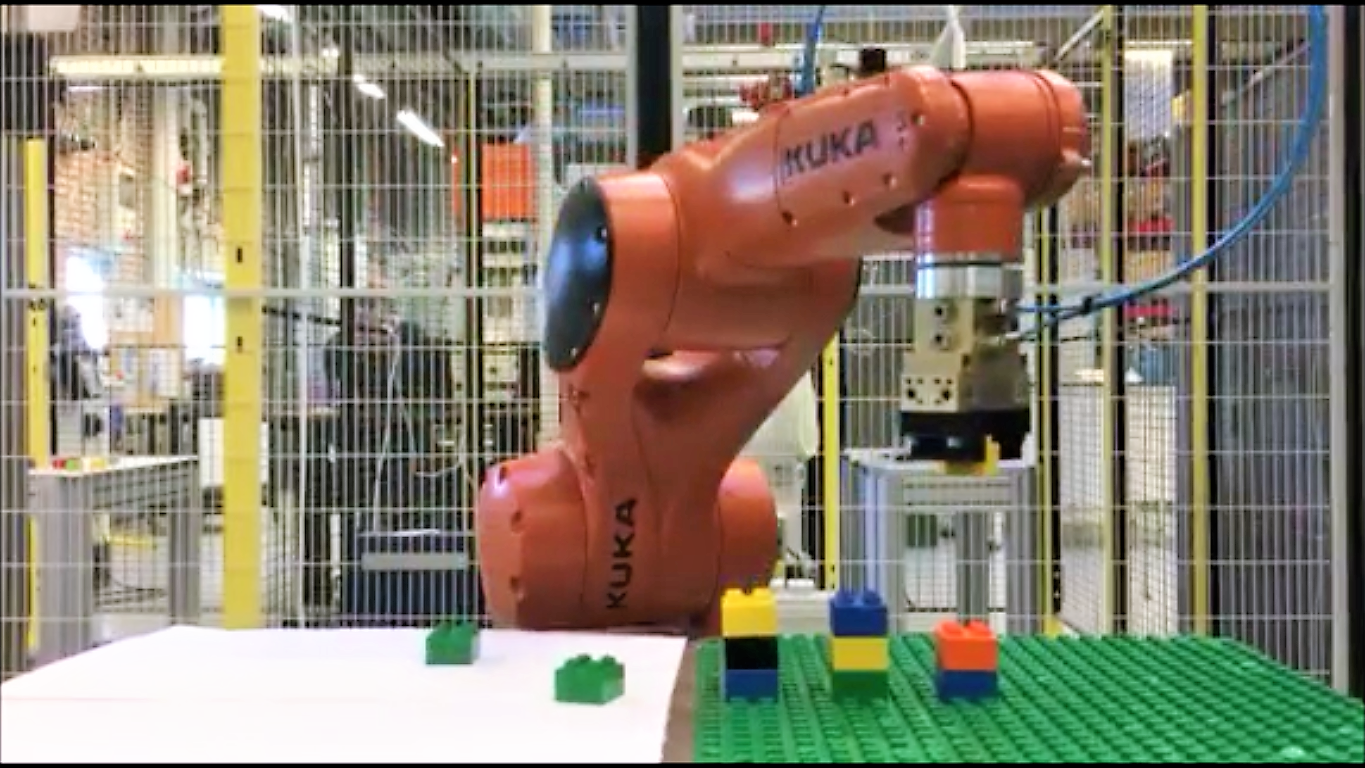
\includegraphics[width=0.5\textwidth]{figures/results.png}
    \caption{Frame of one of the demo videos.}
    \label{fig:results}    
\end{figure}

In this miniproject, Lego bricks have been identified using images from a camera, resulting in the position, orientation and color of each brick. The vision algorithm was based on color segmentation in HSV color space, object analysis, edge detection and Hough transform for lines. The information was then transformed into workspace coordinates through a projection matrix, which was obtained by correspondence between pairs of points.

The algorithm that moved the robot was composed by pick and place operations. These were defined by the desired figures to be built and its final position and orientation and the information of the bricks coming from the vision algorithm.